\section{Introduction}

JOpenShowVar is a versatile, open-source communication 
interface written in Java, designed to be cross-platform. 
It facilitates the reading and writing of all variables 
associated with a controlled manipulator. 
While it is primarily suited for soft real-time applications, 
JOpenShowVar offers significant flexibility for researchers. 
It supports the integration of various input devices and sensors, 
which can be used to explore and develop novel control 
methodologies. The library is highly compatible, 
functioning seamlessly with all Kuka industrial robots that 
utilize either the KR C4 or KR C2 controllers. 
This makes JOpenShowVar an invaluable tool for experimentation 
and innovation in robotic control systems, enabling the 
implementation of alternative control strategies and the 
advancement of research in automation and robotics.\cite{sanfilippo2015controlling}
\\ KUKAVARPROXY is a robust multi-client server capable of 
serving up to 10 clients simultaneously. 
It implements the KUKA CrossComm class, 
which provides a wide range of functionalities essential for 
controlling and managing KUKA robots. 
These functionalities include selecting or canceling 
specific programs, detecting errors and faults, 
renaming program files, saving programs, resetting I/O drivers, 
as well as reading and writing variables.\cite{sanfilippo2015controlling}
\\ The communication protocol between KUKAVARPROXY and 
JOpenShowVar utilizes TCP/IP, specifically through the 
exchange of specially formatted strings on the TCP/IP layer. 
\\ KUKAVARPROXY actively listens on TCP port 7000, awaiting 
connections. Once a connection is established, the server is 
prepared to handle any read or write requests from the client. 
This setup allows for efficient and reliable message exchange 
between KUKAVARPROXY and JOpenShowVar, facilitating seamless 
communication and control over the robotic systems.\cite{sanfilippo2015controlling}

\begin{figure}[h]
    \centering
    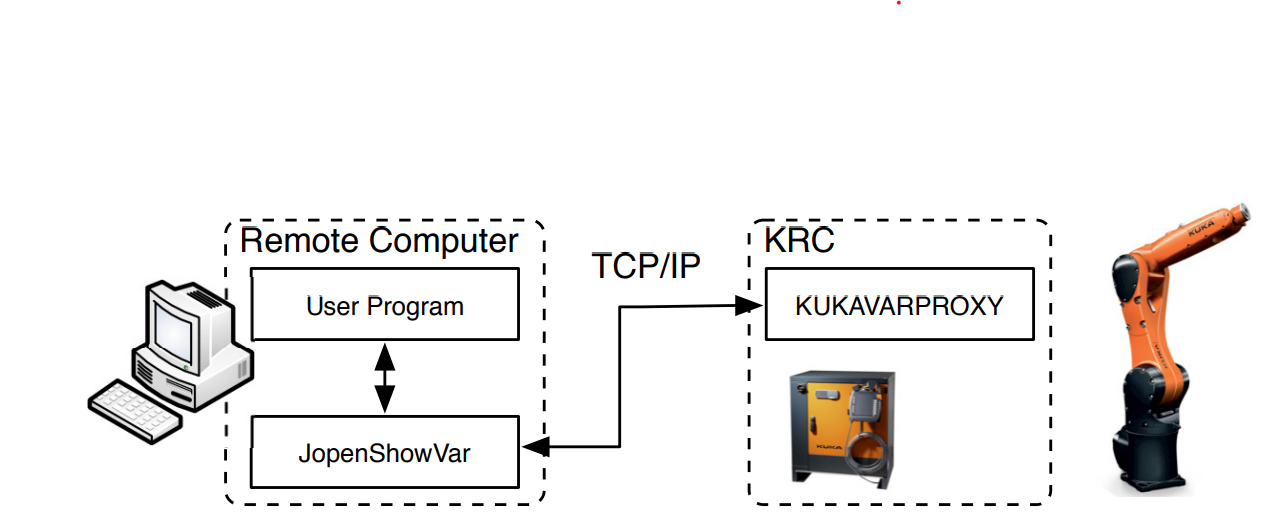
\includegraphics[width=0.9\textwidth]{KVP}
    \caption{architecture of JOpenShowVar}
    \label{fig:mesh1}
\end{figure}